\section{Internal Combustion Engine Simulator}
%
ICESym es un simulador de motores de combustión interna que  utiliza modelos 0D
para la cámara de combustión y 1D para el flujo a través del sistema de
intercambio de gases.
%
Esta combinación permite evaluar la \emph{performance} de un motor a un costo
computacional relativamente bajo; además la implementación de entrada y salida
de datos facilita utilizar el simulador como una \emph{caja negra}.
%
Esta característica permite incluir al simulador en un \emph{script} como una
función, a la cual se le otorga un conjunto de parámetros de entrada y devuelve
los resultados de la simulación en un formato que permite la lectura y
evaluación de los mismos.

ICESym contiene en su código las rutinas necesarias para simular el ciclo
operativo y la geometría del MRCVC.
%
Se realizaron modificaciones menores para facilitar la ejecución en conjunto con
el optimizador, algunas de estas modificaciones fueron:
%
\begin{enumerate}
    \item Modificar el formato de los archivos de salida, con el fin de reducir
el tamaño de los archivos de salida, facilitar la lectura y el procesamiento de
datos.
    \item Incluir una opción para elegir entre un modelo de $C_D$ de una o dos
variables.
    \item Modificar el área de referencia, ver ec.\ref{ec:fv}
    \item Agregar un esquema de interpolación bilineal que permita tabajar con
el modelo de $C_{D}$ de dos variables.
\end{enumerate}


\section{Modificaciones a ICESym}
%%%%%%%%%%%%%%%%%%%%%%%%%%%%%%%%%%%%%%%%%%%%%%%%%%%%%%%%%%%%%%%%%%%%%%%%%%%%%%%
\subsection{Flujo a Través de los Puertos}
%
Se introdujo una opción para poder ejecutar ICESym con un modelo del coeficiente
de descarga que dependa de dos variables: diferencia de presión y \emph{alzada}
o apertura del puerto, $C_D = f(lv; \Delta P)$.
%
Esto significó agregar un \emph{switch} en el código que permita seleccionar
entre un modelo de una o dos variables, con el agregado de las instrucciones de
lectura de datos y armado de un arreglo bidimensional que contiene los valores
del mapa de $C_{D}$ en un orden dado.
%
Con esto se construye un mapa del coeficiente de descarga de la forma $C_D =
f(lv, \Delta P)$, que se utiliza para calcular el área efectiva del puerto.

\nomenclature[F]{\(\Delta P\)}{Diferencia de presión a través de un puerto}


Independientemente de la cantidad de variables que formen parte del coeficiente
de descarga, a ICESym se introduce un vector para el caso 1D y matriz para el
caso 2D.
%
El esquema de interpolación bilineal implementado requiere de una malla
rectangular, se reutilizó el código existente para el caso 1D y se realiza una
interpolación lineal entre dos valores en planos con datos conocidos, como se ve
en la Figura~\ref{fig:interp_bilineal}.

\begin{figure}
    \centering
    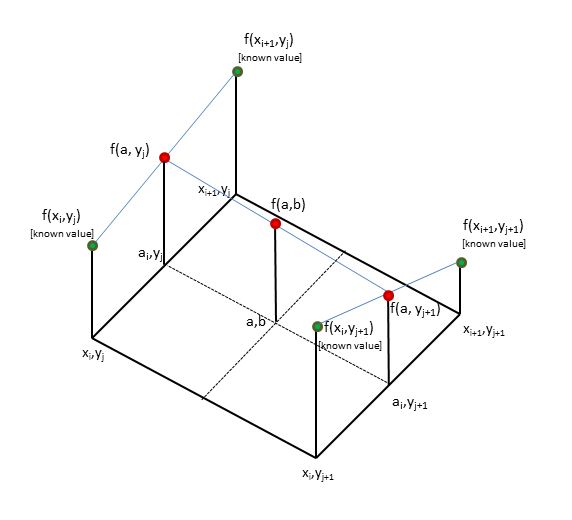
\includegraphics[width=0.7\textwidth]{interpolacion_bilineal.png}
    %
    \caption{Interpolación bilineal\protect\footnotemark}\label{fig:interp_bilineal}
    % \footnote{A}}
\end{figure}

\footnotetext{\url{https://stackoverflow.com/questions/8808996/bilinear-interpolation-to-enlarge-bitmap-images}}

Si bien hay otros métodos de interpolación para estimar el valor de $C_D$ a
partir de una nube de puntos, este método es sencillo y da resultados
satisfactorios.
%
En la Figura~\ref{fig:bilineal} se muestra a modo de ejemplo del error obtenido
con este método para interpolar una función de prueba
$f=\sin\left(\sqrt(x^2 + y^2)\right)$.

\begin{figure}
    \centering
    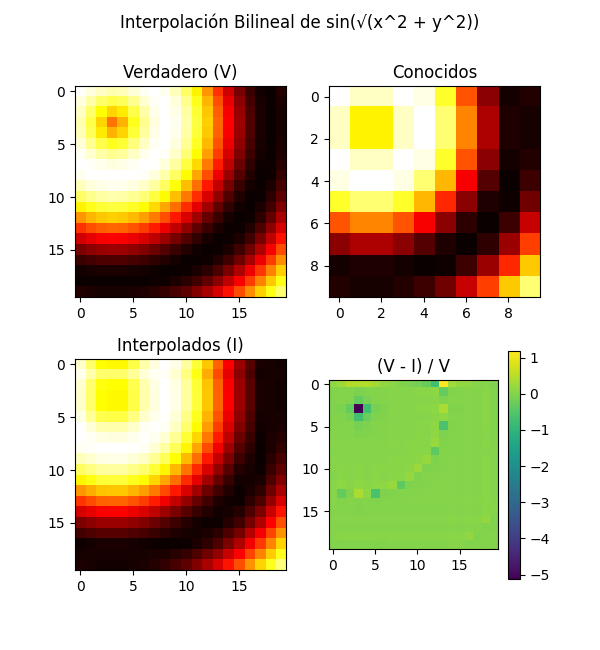
\includegraphics[width=0.7\textwidth]{bilineal.png}
    \caption{Interpolación bilineal de $\sin(\sqrt(x^2 + y^2))$}\label{fig:bilineal}
\end{figure}

La malla rectangular requerida para la interpolación bilineal del mapa de
$C_{D}$ se realizará a partir de los valores resultantes de las flujometrías con
\emph{OpenFOAM}~\parencite{openfoam}.
%
Debido al costo computacional que requieren las flujometrías, solo una cantidad
reducida de puntos se obtendrá con este método.
%
Se tiene como punto de partida una malla no rectangular, por lo que se utiliza
un método intermedio para obtener una matriz de puntos que pueda ser leída por
la interpolación bilineal.

Se probaron dos métodos para realizar la interpolación, el método del punto más
cercano (MC) y la interpolación por la suma de la inversa de la distancia o IDW por
sus siglas en inglés (\emph{Inverse Distance Weighting}).
%
Estos se combinan con métodos de suavizado de promedio móvil con los $S$ valores
más cercanos, con este método cada valor original de la matriz se reemplaza por
el promedio aritmético de los valores a $S$ filas o columnas de distancia.
%
En la Figura~\ref{fig:suavizado_promedio} se muestra este proceso para una
matriz $5\times5$.

\begin{figure}
    \centering
    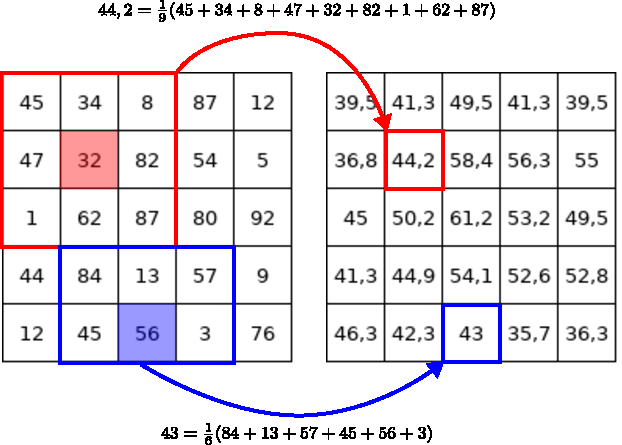
\includegraphics[]{/mapa_cd/suavizado.pdf}
    \caption{Suavizado por promedio con celdas vecinas, S=1}\label{fig:suavizado_promedio}
\end{figure}


El método del punto más cercano consiste en asignar para cada par $(x, y)$ el
valor conocido más cercano, ver Algoritmo~\ref{algo:mas_cercano}.

\begin{algorithm}
 \caption{Interpolación por punto más cercano}\label{algo:mas_cercano}
    \KwIn{\\
        $V_x, V_y$: valores de $x, y$ en los que se conoce el valor en $z$.\\
        $V_z$: valores conocidos de $z$.\\
        $I_x$: $n$ puntos de $x$ donde se quiere interpolar\\
        $i_y$: $m$ puntos de $y$ donde se quiere interpolar\\
        }

    \KwResult{Devuelve una matriz $I_{[n,m]}$ con los valores interpolados,
      donde a cada punto $I(x,y)$ se le asigna al valor de $v_z$ más cercano
      conocido. Da como resultado superficies escalonadas.}

    \BlankLine
     $I=zeros_{[n,m]}$\;
     \For{$i \gets 0$\KwTo$n$}{
        \For{$j \gets 0$\KwTo$m$}{
          $d = \sqrt{{(V_x - I_{xi})}^2 + {(V_y - I_{yj})}^2}$\;
            $I[i,j] = v_z[\min(d)]$\;
        }
     }
\end{algorithm}

La interpolación por IDW consiste en asignar a cada punto el resultado de un
promedio de los valores cercanos, ponderado por la distancia elevado a un
exponente arbitrario $p$.
%
Cuanto más grande el valor de $p$, más sensible es el método a los valores
cercanos.
%
La ecuación del promedio es la~(\ref{eq:idw}) y en el Algoritmo~\ref{algo:IDW}
se presenta el esquema utilizado.
%
En la Figura~\ref{fig:mapas_interpolados} se muestra una comparación de ambos
métodos, para una malla de $C_{D}=f(\Delta_{P}, l_{v})$ generada al azar.

\begin{equation} \label{eq:idw}
    f_p = \frac{\sum_{i=1}^{n} \frac{z_i}{d_i^p}} {\sum_{i=1}^{n}
    \frac{1}{d_i^p}}
\end{equation}

\begin{algorithm}
    \caption{Interpolación IDW}\label{algo:IDW}
    \KwIn{\\
        $V_x, V_y$: valores de $x, y$ en los que se conoce el valor en $z$.\\
        $V_z$: valores conocidos de $z$.\\
        $I_x$: $n$ puntos de $x$ donde se quiere interpolar\\
        $i_y$: $m$ puntos de $y$ donde se quiere interpolar\\
        $p$: potencia a la que se eleva cada peso\\
        }

    \KwResult{Interpolación ponderada por inverso de la distancia. Dependiendo
      del valor de $p$, se obtienen valores más o menos suavizados.}

    \BlankLine
    $I=zeros_{[n,m]}$\;
    \For{$i \gets 0$\KwTo$n$}{
        \For{$j$\gets 0 \KwTo$m$}{
          $d = {\left[{(V_x - I_{xi})}^2 +{(V_y - I_{yj})}^2\right]}^{\frac{p}{2}}$\;
          \eIf{$\exists i : d[i] = 0$}{
            $I[i, j] = V_z[i]$\;
          }{
            $I[i,j] = \frac{\sum{V_{zi}/d_i}}{\sum \frac{1}{d}}$\;
          }
        }
     }
\end{algorithm}


\begin{figure}
    \centering
    \begin{subfigure}{0.4\textwidth}
        \centering
        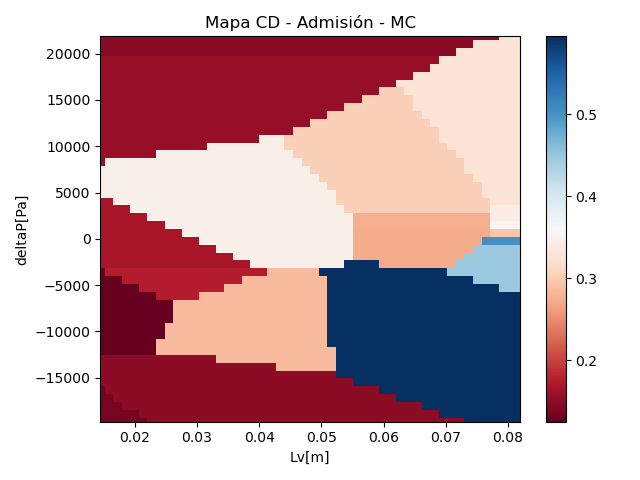
\includegraphics[width=\textwidth]{mapa_cd/mc_mapa_adm.png}
        \caption{Punto Más Cercano sin suavizar}
    \end{subfigure}
    \hfill
    \begin{subfigure}{0.4\textwidth}
        \centering
        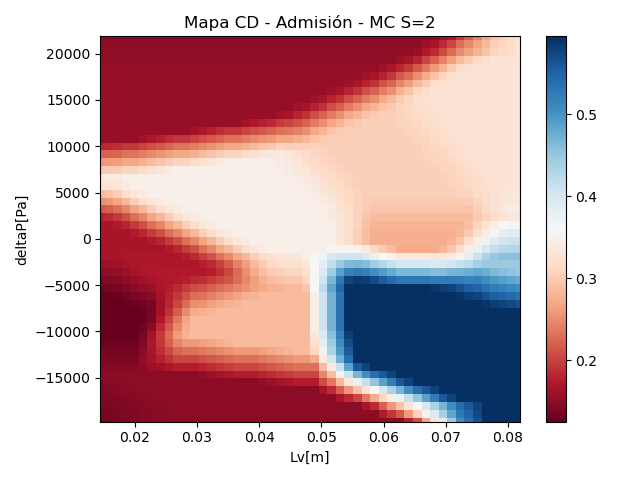
\includegraphics[width=\textwidth]{mapa_cd/mc_s2_mapa_adm.png}
        \caption{Más Cercano ($S=2$)}
    \end{subfigure}
    \hfill
    \begin{subfigure}{0.4\textwidth}
        \centering
        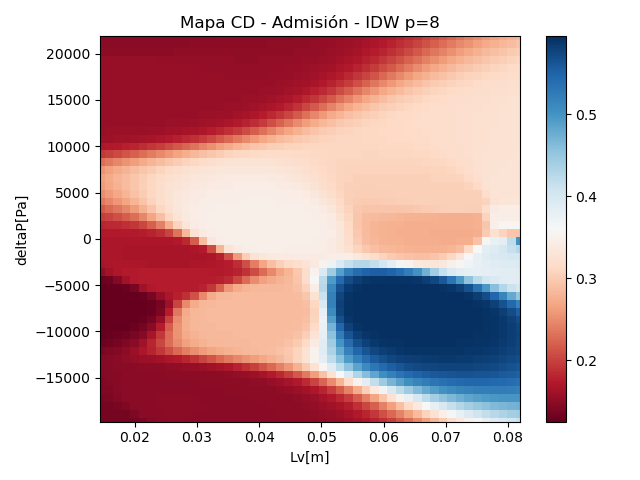
\includegraphics[width=\textwidth]{mapa_cd/idw8_mapa_adm.png}
        \caption{IDW ($p=8$)}
    \end{subfigure}
    \hfill
    \begin{subfigure}{0.4\textwidth}
        \centering
        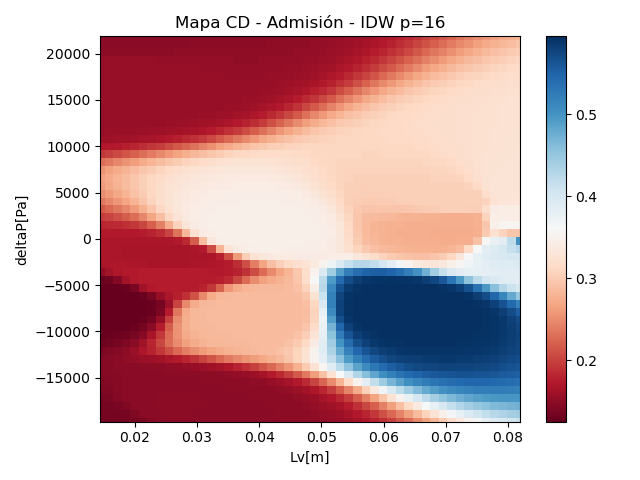
\includegraphics[width=\textwidth]{mapa_cd/idw16_mapa_adm.png}
        \caption{IDW ($p=16$)}
    \end{subfigure}
    \caption{Comparación de interpolaciones}\label{fig:mapas_interpolados}
\end{figure}

%%%%%%%%%%%%%%%%%%%%%%%%%%%%%%%%%%%%%%%%%%%%%%%%%%%%%%%%%%%%%%%%%%%%%%%%%%%%%%%

\subsection{Área de Referencia}
%
El área de referencia utilizada por ICESym es el área de
cortina~(\ref{eq:area_cortina}) y se expresa en el código del programa como el
área efectiva $F_{V}=A_{R}\cdot C_{D}$.
%
Como se indicó en el apartado~\ref{sec:cap2_cd}, para el  MRCVC el área de
referencia es el área frontal del puerto expuesta a la cámara, calculada como la
altura de la ranura $h_{p}$ multiplicada por la distancia entre el borde del
puerto y la paleta que delimita la cámara, denominada como $l_{v}$.

%
% En la Figura~\ref{fig:area_referencia} se ilustran las áreas de referencia para
% una posición del rotor en la que hay solape de cámaras con $\theta = 55^\circ$.
%
Este valor se afecta por el coeficiente de descarga intermedio $C_{D,int}$, que
puede ser un valor fijo o el resultado de interpolar de un mapa de $C_D$ para un
valor de cuerda y $\Delta_P$ dado, como se indica en la ecuación~(\ref{eq:fv}).

\begin{equation}\label{eq:fv}
    F_v = C_{D,int}\cdot h_{p}\cdot l_{v} = 0,0294\cdot C_{D,int}\cdot l_{v}
\end{equation}

% \begin{figure}
%     \centering
%     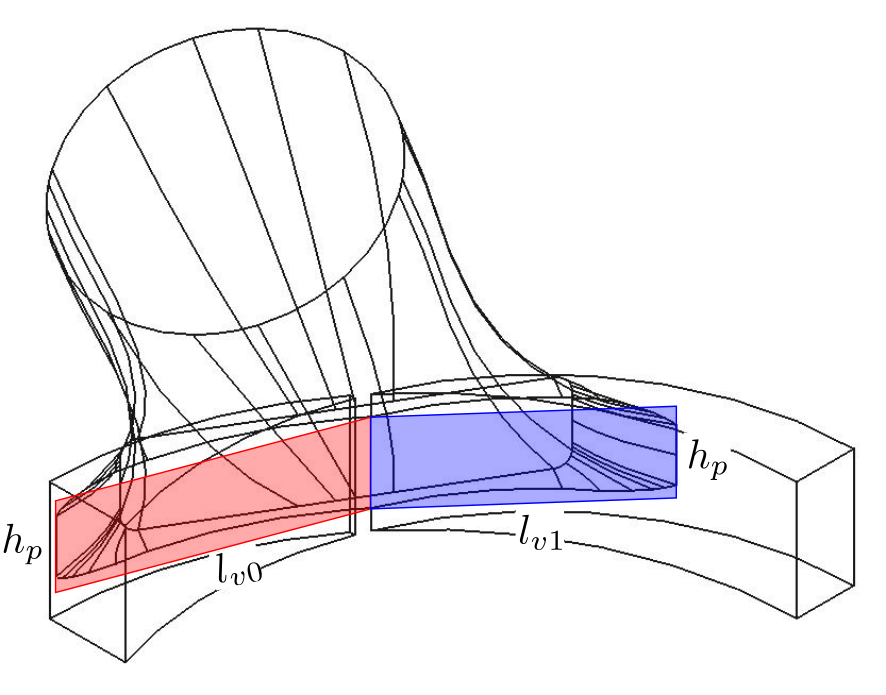
\includegraphics[]{area_referencia.png}
%     \caption{Área de referencia}\label{fig:area_referencia}
% \end{figure}

Tanto al inicio como al cierre del puerto ocurre solape de cámaras, por lo que
en estos intervalos angulares hay un valor de $C_D$ para cada cámara.
%
Este se calcula con el flujo másico que atraviesa las secciones de entrada
correspondientes a cada cámara y el área de puerto expuesta por cada cámara.

\subsection{Interfaz con Optimizador}
%
Para lograr ejecutar el simulador automáticamente, se creó una librería de
funciones capaz de tomar como dato de entrada un archivo de configuración que
incluye geometría, velocidades a ejecutar y cantidad de ciclos de simulación,
entre otros.

Para ejecutar una instancia de ICESym se puede utilizar la interfaz gráfica de
usuario (GUI) ó ejecutarlo por línea de comando desde una consola.
%
El simulador de motores se ejecuta como un archivo de Python {\tt>> python
main.py}, elc ual archivo contiene las instrucciones que lanzan la simulación del
motor con una configuración dada.
%

ICESym requiere de un archivo de configuración con los datos de la simulación a
realizar, este archivo se organiza como sigue:

\begin{forest}
  [config.py
    [Atmospheres]
    [Junctions]
    [Simulator]
    [Cylinders
      [Combustion]
      [Fuel]
      [Inyection]
      [Valves]]
    [Tanks]
    [Tubes]
  ]
\end{forest}

\begin{itemize}
  \item {\tt Atmospheres}: contiene el estado de la atmósfera, que es condición de
contorno de la simulación: presión, densidad y velocidad inicial.
  \item {\tt Cylinders}: geometría y condiciones de contorno, estado inicial,
combustible, como así también de las válvulas.
  \item {\tt Valves}: geometría, tipo de válvula, modelo de $C_{D}$, perfil de alzada y
datos de $C_{D}$ y tubo conexionado.
  \item {\tt Junctions}: contiene información de las uniones entre tubos.
  \item {\tt Simulator}: configuración de la simulación, velocidades a simular,
propiedades de gas, combustible, directorios, entre otros.
  \item {\tt Tanks}: volumen, masa y temperatura de pared de tanques.
  \item {\tt Tubes}: geometría, cantidad de nodos y conexiones.
\end{itemize}

Los elementos de configuración intervenidos por el optimizador son {\tt
Cylinders}, {\tt Valves} y {\tt Simulator}; donde se pueden modificar según
necesidad los siguientes valores:

\begin{itemize}
  \item {\tt Simulator}:
        \begin{itemize}
          \item {\tt RPMS}: Velocidades a simular (por ejemplo una lista de [1000,
2000, \ldots, 9000).
          \item {\tt NCYCLES}: cantidad de ciclos por velocidad (un entero mayor o igual a 1).
          \item {\tt FOLDER NAME}: nombre de la carpeta donde se guardan los
resultados de la simulación.
          \item {\tt SHOW INFO}: selector para mostrar o no información de la simulación.
          \item {\tt CONFIG DATA}: archivo donde se guarda la configuración utilizada.
        \end{itemize}
  \item {\tt Cylinders} $\longrightarrow$ Valves
        \begin{itemize}
          \item {\tt LvI}: perfil de alzada del puerto de admisión.
          \item {\tt LvE}: perfil de alzada del puerto de escape.
          \item {\tt IPO}: ángulo de apertura del puerto de admisión.
          \item {\tt IPC}: ángulo de cierre del puerto de admisión.
          \item {\tt EPO}: ángulo de apertura del puerto de escape.
          \item {\tt EPC}: ángulo de cierre del puerto de escape.
          \item {\tt cd\_model}: selector de modelo de $C_{D}$.
                \begin{itemize}
                  \item $C_{D}l_{v}$ valores de alzada para el mapa de $C_{D}$(
para modelo de 2 variables).
                  \item $C_{D}d_{p}$ valores de $\Delta_{P}$ para el mapa de
$C_{D}$ (para modelo de 2 variables).
                  \item $C_{D}$ valores de $C_{D}$ relacionados con alzada (para modelo de 1 variable).
                \end{itemize}
          \item $D_{v}$: diámetro de la cabeza de la válvula.
        \end{itemize}
  \item Tubes
        \begin{itemize}
          \item longitud: longitud total del tubo de admisión o escape.
        \end{itemize}
\end{itemize}
